\documentclass[12pt]{report}   % list options between brackets
\usepackage{titlesec}
\usepackage{hyperref}
\usepackage[margin=1.25in, footskip = 0.5in]{geometry}
\usepackage{graphicx}
\usepackage{subcaption}
\usepackage{placeins}
\usepackage{apacite}
\usepackage{caption}

\titleformat{\chapter}[display]
{\normalfont\huge\bfseries}{}{20pt}{\Huge}   
\titlespacing*{\chapter}{0pt}{-50pt}{40pt}

\titleformat{\title}
	{\Large\bfseries}{}{0pt}{\huge}

% type user-defined commands here

\begin{document}

\title{%
Topic-Sensitive Submitter Ranking:\\[0.3em]
\large Application of the PageRank Algorithm for Inference of Submitter Interests}   % type title between braces
\author{Anna Marbut}         % type author(s) between braces
\date{May 2019}    % type date between braces
\maketitle


\chapter*{Abstract}
\label{abstract}
\addcontentsline{toc}{chapter}{\nameref{abstract}}

Submittable is a software-as-a-service company that provides a platform for companies to seamlessly receive and review file submissions. In addition to its main product, Submittable also offers client companies the option of running a marketing campaign for specific submission opportunities. As part of these marketing campaigns, Submittable needs to create lists of submitters who are likely to be interested in any given opportunity, but lacks explicit input from users about their interests. Here, Google's PageRank algorithm is adapted to create a list of users ranked in order of their inferred interest in an opportunity. Topic scores are created for opportunities and users based on a weighted count of opportunity-specific keyword matches. These scores are then used to create topic-specific similarity scores between all pairs of users, which feed the iterative process of a PageRank adaptation, here termed SubmitterRank. Random samples of 500 and 5000 Submittable users were used as a proof-of-concept, and coarse comparison to straight keyword-matching suggests that the algorithm is performing as expected and may indicate improvement on keyword-matching alone. Future directions include exploration of a distributed computing solution to run the algorithm on the entire dataset and various options for quantifying performance of a list created from the entire dataset using SubmitterRank.


\tableofcontents

\chapter{Introduction}

Submittable was founded in 2010 by three software developers who were creatives when they were off the clock -- one novelist, one musician, and one filmmaker. All three had experience with the submission process for creative work, and saw a need for improvement. This process varied for every opportunity: one organization might want to be mailed a physical copy of the work, another might want to be mailed a thumb drive, another might receive submissions via e-mail, and yet another might use a digital filesharing service. In exploring possible solutions for their own frustrations, Submittable's founders quickly realized how much worse it was for the organizations receiving the submissions. These organizations were using physical filing systems, spreadsheets, e-mail chains, and any number of other quasi-structured methods to track the submissions that they'd received and the various communications, review processes, and administrative tasks related to them. This left a lot of room for human error and increased frustration on both sides of the whole process.

With these issues in mind, Submittable's founders set out to create a platform which could accept all of the most common filetypes (even very large files) and streamline the entire submission management pipeline. Almost 10 years later, Submittable has helped 15 thousand organizations collect and manage over 12 million submissions. While the bulk of their clients remain in the creative realm (literary journals, film contests, photography journals, auditions, etc.), they have branched out into almost every industry in which any type of submission needs to be made (research grants, job applications, charitable foundations, residency programs, etc.), and the number of these other clients is growing quickly. The company has grown from three founders to 70 employees, was picked up by the startup incubator Y-Combinator (known for DropBox, AirBnB, Weebly, and others), and has received over \$5 million in venture capital funding. 

Submittable's business model has been one of ``software-as-a-service", or SAAS, in which their clients pay a subscription fee for use of the software platform. Different subscription levels are available based on which features each organization wants to use. Available features include the number of active opportunities allowed (also referred to as ``calls to submission" or ``forms"), the option for multiple reviewers, gallery voting (such as for public photography contests), submission fee collection, and automated reporting. As the business has grown, the features offered to client organizations have expanded from those immediately related to software functionality, to more abstract features such as hosting an opportunity on a custom url, white-labelling the software, or providing marketing services to promote a specific opportunity or organization. This last feature is the inspiration and focus for this project.

When a client opts for a subscription package that includes marketing services, they work with Submittable's marketing team to design a custom campaign for the client's opportunities. This campaign can consist of social media outreach, blog posts, newsletter articles, and/or custom reminders to interested submitters. Almost always, a marketing campaign also includes an e-mail campaign to a targeted list of Submittable's users (aka submitters). Currently, these lists are populated by matching users based on the use of campaign-specific keywords in their personal description, submission cover letter, or in the description or name of opportunities to which they've submitted. While this method makes a pretty good guess at which submitters would be interested in the campaign, it is a broad way to segment the submitter base, and is likely to both include some submitters who won't be interested and leave out some who would be. 

In this project, we will explore using an adaptation of the PageRank algorithm to rank submitters based on their interest in a specific topic. The goal is to provide Submittable with a more robust method for selecting which submitters should be contacted for a specific marketing campaign. Improving the quality of these lists will improve the experience for both client and submitter, with clients reaching users and receiving submissions that are a better fit for their opportunities, and submitters receiving promotions about opportunities to which they are more likely to submit. Resource limitations for this project necessitate the use of random sampling to first perform a proof-of-concept for these methods, with future work leading to the application of the PageRank adaptation on the entire dataset of submitters.

\chapter{Data and Descriptive Statistics}         
\section{Data Source}
The data for this project come from an Amazon Redshift Database that Submittable has set up to perform basic analytic queries about their clients, users, and product usage. Due to the scope of this research, the data used is centralized around Submittable's users, including information that they've explicitly provided on their Submittable profile, as well as information about the various submissions that they've made. In accordance with Submittable's privacy policy, no information that could be used to identify an individual user was included in the data for this project.

\section{User Accounts}
Submittable has 4.2 million users from all time, 770 thousand of whom made a submission in 2018. As seen in Figure \ref{fig:userCreate}, the number of new user accounts has increased exponentially, with almost twice as many new accounts in 2018 as there were in 2017. The number of users making at least one submission is also increasing steadily each year, although on a linear scale with about 100 thousand more active submitters each year since 2013 (Figure \ref{fig:userSubmit}). On average, Submittable users have made five submissions in their account lifetimes, with the number of submissions that an individual user has made ranging from one to 7.4 thousand. Additionally, 62\% of Submittable users have only made one submission since they created their account.
\begin{figure}[h]
    \centering
    \begin{minipage}{0.45\textwidth}
	  \captionsetup{font=scriptsize}
        \centering
        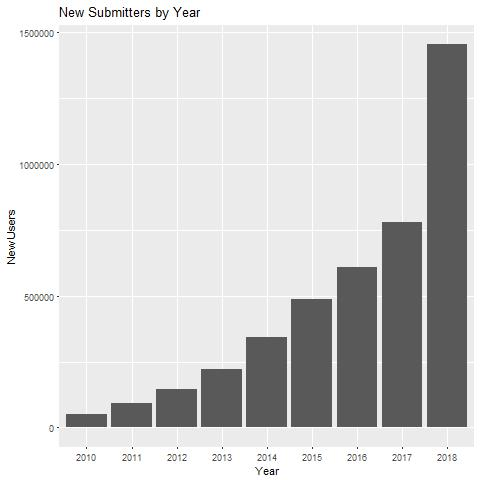
\includegraphics[width=1\textwidth]{userCreate_plot.jpg} % first figure itself
        \caption{New Submittable User Accounts by Year}
	  \label{fig:userCreate}
    \end{minipage}\hfill
    \begin{minipage}{0.45\textwidth}
	   \captionsetup{font=scriptsize}
        \centering
        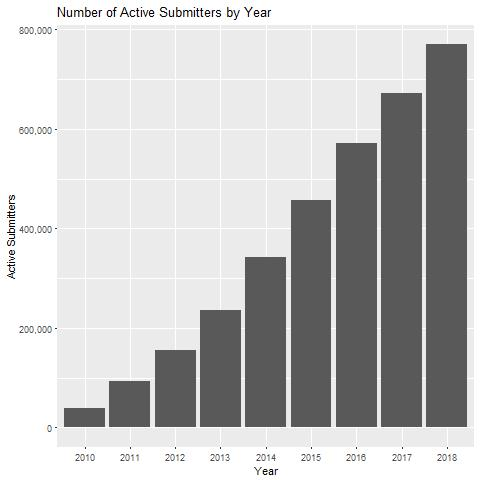
\includegraphics[width=1\textwidth]{userSubmit_plot.jpg} % second figure itself
        \caption{ Submittable Users with at least One Submission by Year}
	  \label{fig:userSubmit}
    \end{minipage}
\end{figure}
\FloatBarrier
In creating a Submittable account, each submitter has the option to provide a written description of themselves. Roughly 100 thousand submitters have something written in their description field, and a brief scan shows that these are fairly descriptive, like what would be included in a cover letter or a professional biography. 1.2 million of Submittable's users have also provided location information, hailing from 244 countries and territories. 75\% of these users are from the United States, and 91\% of them are from the top ten countries shown in Table \ref{table:userCountry}. 

\begin{figure}[h]
\centering
\begin{minipage}{0.45\textwidth}
	\captionsetup{font=scriptsize}
     \centering
\captionof{table}{Top Ten Submittable Users' Countries}
\label{table:userCountry}
\begin{tabular}{rlr}
  \hline
 & Country & Number of Submitters \\ 
  \hline
1 & United States & 913542 \\ 
  2 & United Kingdom & 59268 \\ 
  3 & Canada & 56316 \\ 
  4 & Australia & 26898 \\ 
  5 & India & 22709 \\ 
  6 & Nigeria & 7458 \\ 
  7 & Germany & 7359 \\ 
  8 & France & 5652 \\ 
  9 & South Africa & 5578 \\ 
  10 & Italy & 5451 \\ 
   \hline
\end{tabular}
    \end{minipage}
\end{figure}
\FloatBarrier

\section{Opportunities and Submissions}
Submittable's software platform has hosted a total of almost 130 thousand opportunities, with a fairly steady increase of 3-5 thousand new opportunities created every year except for 2018 (Figure \ref{fig:formYear}). This decrease in new opportunities last year can likely be attributed to the maturation of many client accounts, who are now re-using forms that they've created in previous years. This is also supported by the steady increase in the total number of submissions made each year, including last year, which has increased by about 300 thousand every year since 2010 (Figure \ref{fig:subYear}). In its lifetime, Submittable has received a total of 12 million submissions.

\begin{figure}[h]
    \centering
    \begin{minipage}{0.45\textwidth}
	\captionsetup{font=scriptsize}
        \centering
        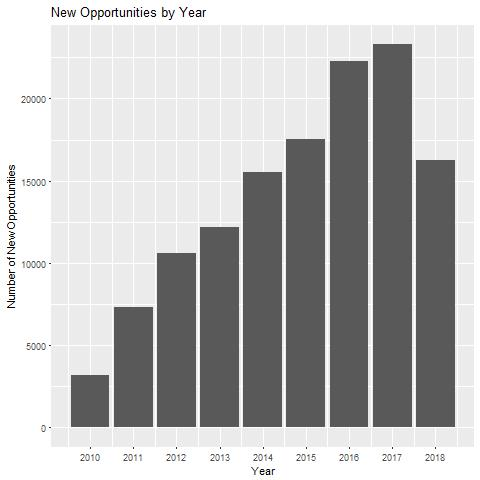
\includegraphics[width=0.9\textwidth]{formsByYear_plot.jpg} % first figure itself
        \caption{ New Submittable Opportunities by Year}
	  \label{fig:formYear}
    \end{minipage}\hfill
    \begin{minipage}{0.45\textwidth}
	\captionsetup{font=scriptsize}
        \centering
        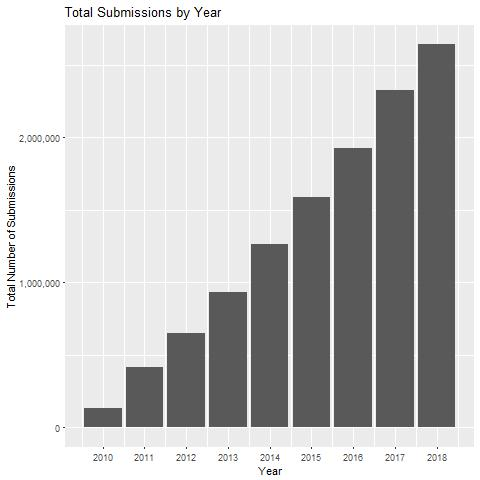
\includegraphics[width=0.9\textwidth]{subsByYear_plot.jpg} % second figure itself
        \caption{Total Number of Submissions Made by Year}
	  \label{fig:subYear}
    \end{minipage}
\end{figure}
\FloatBarrier
On average, opportunities that have received at least one submission have received 125 submissions, with a range from one to 145 thousand. About 75\% of opportunities have received at least one submission, 45\% have received at least five submissions, and 30\% have received over 20 submissions. The intermittent nature of many opportunities makes it difficult to define what should be considered an ``active" opportunity, but Figure \ref{fig:activeForms} shows the number of opportunities that received at least one submission each year. These numbers follow a similar, though less dramatic, pattern as the number of new opportunities each year (Figure \ref{fig:formYear}), steadily increasing until 2018.

\begin{figure}[h]
    \centering
    \begin{minipage}{0.45\textwidth}
	\captionsetup{font=scriptsize}
        \centering
        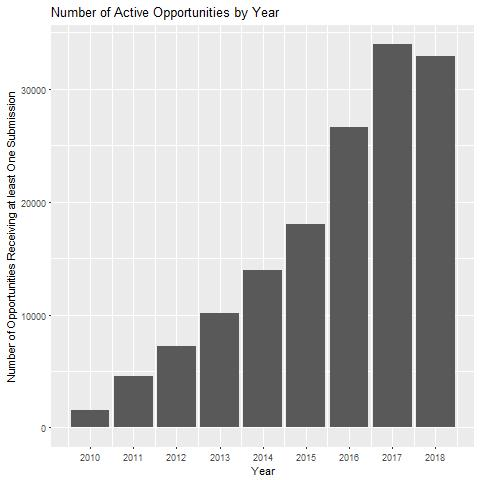
\includegraphics[width=0.9\textwidth]{activeForms_plot.jpg} % first figure itself
        \caption{Number of Opportunities Receiving at least One Submission by Year}
	  \label{fig:activeForms}
    \end{minipage}\hfill
\end{figure}
\FloatBarrier

Each opportunity has various textual data associated with it, including the opportunity name and a brief description of the opportunity. Opportunity descriptions vary greatly in their descriptive usefulness, with some consisting of multiple paragraphs describing the opportunity guidelines in detail, and others simply stating ``Complete the form below". 


\section{Labels}
As Submittable has grown, it has seen several generations of labeling methodologies. Currently, the only actively-updated labels are ``usecase" labels applied at the organizational level, and ``discover" labels applied at the opportunity level. The usecase labels are assigned by account managers and are meant to describe what type of opportunities the organization will offer, such as ``publishing", ``fellowships", or ``grants". The discover labels are assigned by the organizations themselves as they opt in to Submittable's opportunity search engine (called ``Discover"), and can be anything from a list of almost 200 options that they think submitters might search for in relation to their opportunity. The full lists of usecase and discover labels can be found in Appendix \ref{app:labels}.

Only about 40 thousand opportunities are associated with a usecase label (are hosted by an organization with a usecase label). However, this low number is unsurprising since the labels only started being applied in a consistent manner in 2018, and there were also roughly 40 thousand active opportunities in 2018. The ten usecase labels with the highest number of associated opportunities are shown in Table \ref{table:topusecase}.  

67 thousand discover labels are associated with opportunities, however, since the relationship between the discover label and an opportunity is many-to-one, only 20 thousand unique opportunities are associated with discover labels. Also, since many of the discover labels are overlapping (``book" vs. ``memoir" vs. ``stories"), I needed to map these onto broader category labels. Submittable identified grant applicants, filmmakers, photographers, and writers (with the subcategories of poetry, fiction, and non-fiction writers) as specific areas of interest, so I grouped the discover labels under these categories. Table \ref{table:discovergroup} shows the number of unique forms with discover labels that fall into these categories. Since we know that only 20 thousand unique opportunities are associated with discover labels, this table (which sums to about 40 thousand) reiterates the many-to-one relationship between discover labels and opportunities.
\begin{figure}[h]
\begin{minipage}{0.45\textwidth}
\captionsetup{font=scriptsize}
\centering
\captionof{table}{ Top Ten Usecase Labels}
\label{table:topusecase}
\begin{tabular}{rlr}
  \hline
 & Usecase & Count \\ 
  \hline
1 & Publishing & 10836 \\ 
  2 & Grants & 7406 \\ 
  3 & Contest & 4938 \\ 
  4 & Award/ Nomination & 4283 \\ 
  5 & Exhibition & 2626 \\ 
  6 & Conference & 2342 \\ 
  7 & Festival or Event & 1879 \\ 
  8 & Other & 1631 \\ 
  9 & Fellowship & 1613 \\ 
  10 & Scholarships & 1311 \\ 
   \hline
\end{tabular}
\end{minipage}
\hfill
\begin{minipage}{0.45\textwidth}
\captionsetup{font=scriptsize}
     \centering
\captionof{table}{Grouped Discover Labels}
\label{table:discovergroup}
\centering
\begin{tabular}{rlr}
  \hline
 & Discover Group & Count \\ 
  \hline
1 & Fiction & 9871 \\ 
  2 & Film & 5302 \\ 
  3 & Grant & 3157 \\ 
  4 & Nonfiction & 8311 \\ 
  5 & Photography & 5451 \\ 
  6 & Poetry & 8100 \\ 
   \hline
\end{tabular}
    \end{minipage}
\end{figure}


\chapter{Background}
\section{Classification algorithms}\label{classification}

The task of identifying software users for targeted marketing campaigns can be seen as a combination of market segmentation and ontological user profiling. Market segmentation is the process of splitting potential and current customers/consumers into groups based on common characteristics or behaviors \cite{johnson_1971}. Ontological user profiling is the act of inferring user interests based on user behaviors, attributes, and relationships \cite{middleton_shadbolt_roure_2004}. More simply put, this is a classification problem in which we need to identify users based on their potential interest in a topic (or a specific submission opportunity) without having specific information that indicates their interest in said topic. 

A first attempt at addressing this problem was made using an unsupervised classification technique called k-means cluster analysis. In this technique, observations are mapped into an n-dimensional space, where n equals the number of variables being used to classify them. Observations are then grouped into a pre-determined number of clusters by minimizing one of many possible distance measures between observations\cite{jain_2010}. As such, we attempted to group submitters based on the opportunities to which they had submitted--the theory being that users would submit to similar opportunities based on their interests (ie. filmmakers would submit to film opportunities, writers to writing opportunities, etc.). The data was first run through a dimension reduction technique called singular value decomposition (SVD) to reduce the opportunities from 64 thousand to 561, and then the users were clustered into four, seven, and twelve clusters (these values being hypothesized as a good fit for the data based on diminishing returns of minimizing the sum of squared distances within clusters). However, closer inspection of the clusters didn't identify any meaningful connection between users, likely due to the overwhelming majority of writer-focused submitters and opportunities \cite{marbut_2018}.

Other types of algorithms traditionally used for user classification include Naive Bayes techniques, instance-based learner techniques,  and various types of decision trees \cite{cufoglu_lohi_madani_2009}. A common area of research in this area is the profiling Twitter users based on user behavior, network structure, and language used on the profile and in tweets, which has been done through gradient boosted decision trees \cite{pennacchiotti_popescu_2011} and by application of a stacked support vector machine \cite{rao_yarowsky_shreevats_gupta_2010}. However, all of these techniques share a common flaw in the context of Submittable's user classification, which is that they classify observations into one specific category, while submitters may fall equally into multiple groups. While there are fuzzy classification algorithms that will calculate the probability that an observation falls into each of many categories, and methods like support vector machines can be used to identify membership in multiple groups individually, other issues with the data (including incomplete and fuzzy categorization of submission opportunities) suggested that we look for alternative approaches.

\section{Google PageRank}

With the ultimate goal of creating a list of users who were likely to be interested in a specific opportunity, each user can be assigned a ``topic score" based on the keyword matching method that is currently being used to create marketing services lists. This topic score would consist of weighted points for keyword matches in different fields in the database; for example, a user might get a different number of points for every instance of a keyword in the name and description of an opportunity to which they've submitted, as well as in their user profile description. Using a raw score like this would obviously favor users who have made a lot of submissions, have lengthy profile descriptions, or who happen to submit to opportunities with a lot of text in their descriptions. There are similarity measures which can control for this and standardize the raw scores based on sample size and other parameters, however this topic-scoring method still relies entirely on the presence or absence of keywords. If a film opportunity is named only with the name of a contest (eg. ``2018 Company X Awards") and has a minimal description (eg. ``Please complete the form below and submit your work by June 1. Contact Jane Doe with any questions at 123-456-7890"), it would not contribute to a user's film topic score at all. In addition, since we know that 62\% of users have only submitted to one opportunity, if that one opportunity happens to be the ``2018 Company X Awards", the user will not be included in the list of filmmakers even though they should be.

To control for this issue, we needed to find a way to adjust these user topic scores based on similarity to other users. If user A had only ever submitted to the ``2018 Company X Awards", but user B had submitted to this opportunity and a dozen other film opportunities with high topic scores, user A's score should increase based on this connection to user B. This concept of one user's score affecting the score of other connected users is very similar to the theory behind the Google PageRank algorithm, except with users instead of webpages. 

In PageRank, websites are ranked based on the number of other pages that link to them, but also based on the rank of the pages linking to them \cite{page_brin_motwani_winograd_1999}. This self-referrent ranking system is not an exact match for Submittable's usecase, but the idea that one user's topic score (or topic rank) depends at least in part on the topic score of similar users does solve the problem of missing users as discussed above. Also, applying the PageRank algorithm in this context would result in a ranked list of all users based on their interest in a specific topic, which would allow for more dynamic marketing outreach (users who rank very highly might receive more direct outreach than users with a mid-range interest score), and addresses the fuzzy classification issues discussed in Section \ref{classification}.

Similar uses of the PageRank algorithm include the identification of high-impact social network users for marketing campaigns, creation of a topic-specific rank for websites, and identification of highly influential Twitter users on a specific topic. \citeA{heidemann_klier_probst_2012} explore the application of PageRank to Facebook users based on their network connectivity and level of activity. They show that this algorithm can be used to identify key users for viral marketing campaigns that rely on user activity (posting, re-posting, liking, etc.) to reach their target audience. \citeA{haveliwala_2002}  discuss the addition of a topic-bias to the original PageRank algorithm, so that websites with high topicality are favored when calculating their rank based on external links. Finally, \citeA{weng_lim_jiang_he_2010} use PageRank to rank Twitter users based on their influence in a certain area of interest. This approach combines user connectivity and activity with a user-specific topic score to feed the PageRank algorithm and create a ranked list of Twitter users for a given topic.

The methods used in this project, as outlined below, will use aspects of all three of these studies to infer the strength of submitter interests based on the topicality of the opportunities to which they've submitted and their profile descriptions, as well as their similarity to other submitters.


\chapter{Methodology}

\section{Data Selection}

To reach users who are most likely to be interested in submitting to a new opportunity, Submittable's marketing department is only interested in users who have made more than one submission within the last calendar year. This limits the list of potential submitters to just over 400 thousand, which is much more manageable than the entire user base of 2.4 million. However, due to the nature of these methods, even including only 400 thousand users in the dataset requires 160 billion similarity calculations, which is beyond the capabilities of the hardware I currently use. For this reason, random samples of 500 and 5000 submitters will be used as a proof-of-concept in this project, with plans to investigate distributed computing solutions for full-size implementation in the future.

\section{Basic PageRank}

The PageRank algorithm, as described above, is used to rank websites based on the number and quality of other websites that link to it. The math involved in computing this rank is most easily explained using the ``random surfer" analogy. Given a small network of websites, such as that seen in Figure \ref{fig:demoNet} where each letter represents a website and each arrow a link from that site to another site, a web surfer in this network has a certain probability of moving from site to site using only these links, as seen in Figure \ref{fig:demoProb}. 
\begin{figure}[h]
    \centering
    \begin{minipage}[t]{0.48\textwidth}
	\captionsetup{font=scriptsize}
        \centering
        
\includegraphics[scale=0.8]{Marbut_DemoNetwork.png} % first figure itself
        \caption{Small Network of Websites: Each letter represents one website, and each arrow represents a link from one website to another.}
	  \label{fig:demoNet}
    \end{minipage}\hfill
    \begin{minipage}[t]{0.48\textwidth}
	\captionsetup{font=scriptsize}
        \centering
        
\includegraphics[scale=0.8]{Marbut_DemoMatrix.png} % second figure itself
        \caption{Random Surfing Probabilities: Each column represents the probability of navigating from the column page to all other pages in the network by only clicking on links.}
	  \label{fig:demoProb}
    \end{minipage}
\end{figure}
\FloatBarrier

In order to include the possibility of the web surfer directly navigating to any page in the network without clicking on a link (by typing in the address in the navigation bar, for example), a teleportation or damping factor is added to this matrix of probabilities. This teleportation factor applies an arbitrarily-assigned probability, $d$, of navigating the network via links and a $1-d$ probability of directly navigating to any other page in the network to the original matrix. A common value for $d$ is 0.85, which implies that a user has an 85\% chance of navigating to their next page via a link, and a 15\% chance of navigating to another page directly. If $L$ is our original probability matrix from Figure \ref{fig:demoNet}, and $t$ is an $n$ x $n$ matrix of $\frac{(1-d)}{n}$, this transformation can be expressed by Equation \ref{teleport}, resulting in the new probability matrix $M$ seen in Figure \ref{fig:demoDamp}.
\begin{equation}
\label{teleport}
M=d*L+t
\end{equation}

\begin{figure}[h]
    \centering
    \begin{minipage}{0.9\textwidth}
	\captionsetup{font=scriptsize}
        \centering
        
\includegraphics[width=0.45\textwidth]{Marbut_DemoWDamping.png} % first figure itself
        \caption{Transition Matrix with Damping Factor: Each page's navigation probabilities have been transformed such that there is now an 85\% chance of a user navigating via a link and a 15\% chance of direct navigation to another website (such as by use of the navigation bar).}
	  \label{fig:demoDamp}
    \end{minipage}
 \end{figure}
\FloatBarrier 

The way that this transition matrix $M$ has been constructed allows the use of power iteration to create a unique rank vector for all pages in the network. In other words, $M$ can be iteratively multiplied by the rank vector $r$ such that $r$ will eventually converge to a specific eigenvector with an eigenvalue of one, as expressed in Equation \ref{powerrank}. Due to this iterative process, the final rank of any page will be determined by both the total number and rank of pages linking to it \cite{haveliwala_2002}.
\begin{equation}
\label{powerrank}
r^{i+1}=M*r^{i}
\end{equation}

\section{PageRank Adaptation}

In adapting the PageRank algorithm for the purposes of this project, we will be considering submitters instead of websites, and using the number of opportunities to which both of a pair of users has submitted in place of links between pages. Additionally, a topic-bias will be included for each user and each common submission to create topic-specific ranks for each user in the dataset.

\citeA{haveliwala_2002} add topic-bias to their results by creating a topic-specific personalization vector $\vec{p}$ and weighting the damping factor by this vector on each iteration until convergence is reached, as expressed by Equation \ref{topicrank}. The addition of this topic bias in the damping factor is essentially weighting the probability of random direct navigation by how topical each page is, increasing the probability of navigation to pages that are highly topical. 
\begin{equation}
\label{topicrank}
 r^{i+1}=d*M*r^{i}+(1-d)*\vec{p}
\end{equation}

\citeA{weng_lim_jiang_he_2010} instead create a topic-weighted transition matrix $M$, such that the connection between two Twitter users is determined by the proportion of followers that they have in common and weighted by a topic score for each of those users. In this way, the topic-specific connection between two users is stronger (larger in value) if the followers that they have in common are highly topical. This also allows for the topic-specific rank of Twitter users who may not have a high topic score themselves to be pulled up by a strong topical connection to other highly ranked users.

Here, we will use both of these methods to apply a topic-specific bias to the PageRank algorithm. A personalization vector will be used to weight the damping factor based on a user-specific topic score compiled from each submitter's profile description. In addition, the transition matrix will be adjusted such that the number of opportunities that each pair of submitters has in common is weighted by a topic score for each opportunity based on the presence of topic-specific tags and keywords in its name or description.

\section{Topic Scores and Matrix Formation}\label{scoring}

Although the goal of this project is to move away from keyword matching as the basis for creating Submittable's marketing campaign e-mail lists, a lack of consistent and exhaustive labeling in the data means that we still need to rely on a list of topic-specific keywords in order to create topic scores for users and opportunities. However, as discussed above, using these topic scores in combination with the PageRank algorithm will allow for a richer topic-specific ranking of users, including some who would not necessarily have been identified by keyword matching alone.

A personalization vector $\vec{p}$ for each topic is calculated based on the number of keyword matches present in a submitter's profile description. Each user's topic score, $p_{i}$, starts at one and is incremented by two points for every instance of a word from the topic-specific keyword list in their profile description. After all topic scores are calculated, each user's score is divided by the sum of all the user topic scores such that the vector of scores all sum to one (Equation \ref{vecp_prime}).
\begin{equation}
\label{vecp_prime}
p_{i}'=\frac{p_i}{\sum{\vec{p}}}
\end{equation}

Each opportunity's topic score is calculated by a combination of matching keywords in the form description or name and matching usecase or discover tags. This score starts at one and is incremented by one point for every instance of a word from the topic-specific keyword list in the opportunity's description, by two for every instance in its name, and by two for each topic-specific usecase or discover tag. The initial transition matrix, $L$ is then formed with every user on both axes, and the value for every pair of users being equal to the sum of the topic scores for opportunities to which they both submitted. This value is then divided by the column sum for each user, such that each column sums to one (Equations \ref{pairscore} and \ref{Lmatrix}, where $S$ is the set of topic scores for opportunities to which a given user has submitted).
\begin{equation}
\label{pairscore}
L_{i,j}=\sum{S_i\cap S_j}
\end{equation}
\begin{equation}
\label{Lmatrix}
L_{i,j}' =\frac{L_{i,j}}{\sum{L_i}}
\end{equation}

A damping factor, $d = 0.85$, is then added to the transition matrix $L$ in combination with the topic-specific personalization vector $\vec{p}$ by multiplying $\vec{p}$ by an $n$ x $n$ matrix of ones, $J$, such that each column equals $\vec{p}$ (Equations \ref{Pmatrix} and \ref{Mmatrix}). This method is more similar to the original PageRank algorithm than that used by \citeA{haveliwala_2002} in which the personalization vector is added at each iteration. This choice was made for the sake of simplicity for this project, but we will likely compare both methods in the future to determine which performs better in this context.
\begin{equation}
\label{Pmatrix}
P=((1-d)*\vec{p}*J)^{T}
\end{equation}
\begin{equation}
\label{Mmatrix}
M=d*L+P
\end{equation}

Finally, the transition matrix $M$ is multiplied by a rank vector $\vec{r}$ of length n with all starting values equal to $1/n$. This multiplication is iterated until the values in $\vec{r}$ converge at a limit of $1e10^{-8}$ (Equation \ref{submitterRank}). This final value for $\vec{r}$ is the resulting topic-specific rank of all users in the dataset.
\begin{equation}
\label{submitterRank}
r^{i+1}=M*r^{i} \;\; \;\;\;\;\;(r^{i}-r^{i+1})\rightarrow1e10^{-8}
\end{equation}


\chapter{Results}

After taking a random sample of the eligible submitters, we used a list of filmmaker-based keywords (Table \ref{table:filmkeys}) to create topic scores and apply the methods described above to the sample. This resulted in lists of users equal in length to the sample size, each with a rank which is hypothesized to indicate the user's relative interest in a film-related opportunity. In an attempt to quantify the success of these methods, these ranked lists were compared to lists made from the method currently used at Submittable (users are included and ranked equally if they've submitted to any opportunity which has one or more matching keywords in the opportunity name or description, or if the user has one or more matching keywords in their profile description), and from the raw user-topic scores (users are awarded points as described in Section \ref{scoring}, and ranked based on these raw scores). 

\begin{figure}[h]
\centering
\begin{minipage}{0.45\textwidth}
\captionsetup{font=scriptsize}
\centering
\captionof{table}{Filmmaker Keywords}
\label{table:filmkeys}
\begin{tabular}{rlr}
  \hline
 & Keyword \\ 
  \hline
1 & film \\ 
  2 & video \\ 
  3 & animation \\ 
  4 & CGI\\ 
  5 & screenplay \\ 
  6 & documentary \\ 
  7 & feature length \\ 
  8 & screenwriter \\ 
  9 & shot on mobile\\ 
   \hline
\end{tabular}
\end{minipage}
\end{figure}

\section{500-User Sample}

The resulting lists from our initial, very small, random sample of 500 eligible submitters were very different for the SubmitterRank method and the keyword-matching methods. The current methods identify only about 130 of the 500 submitters who may be interested in film-related opportunities, and of the 100 top-scoring submitters on the SubmitterRank list, only 37 were also included on the keyword-matching lists. We also found basically no correlation between the SubmitterRank and raw topic scores and rank orders ($|r|<0.13$), with no improvement if the variables are log transformed. The random scatter apparent in Figure \ref{fig:500cor_orig} also demonstrates that there is no apparent relationship between the ranks resulting from the SubmitterRank algorithm and the raw topic scores.

\begin{figure}[h]
    \centering
    \begin{minipage}{0.9\textwidth}
	\captionsetup{font=scriptsize}
        \centering
        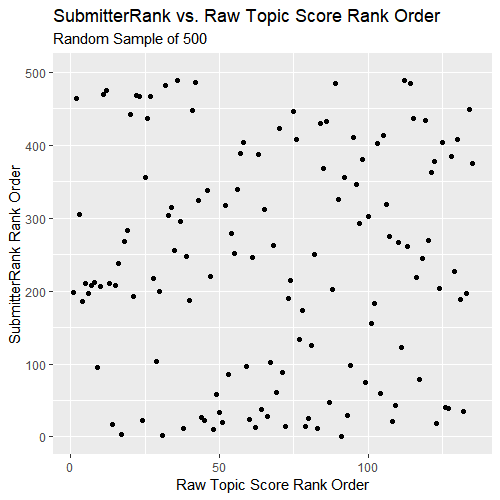
\includegraphics[width=0.45\textwidth]{rankOrder500_orig.png} % first figure itself
        \caption{SubmitterRank vs. Raw Topic Score Rank Orders: Uniform scatter shows no relationship between the raw topic score order and the SubmitterRank order.}
	  \label{fig:500cor_orig}
    \end{minipage}
 \end{figure}

A closer inspection of the highest-ranking submitters in this sample suggests that the keyword-matching method may still be out-performing the SubmitterRank method. Of the five submitters with the highest raw topic scores, three are filmmakers, one is a visual artist, and one doesn't fit neatly into any specific category. The five highest-ranking submitters from the SubmitterRank list consist of two filmmakers, one photographer, and two writers. However, since we know that the majority of Submittable's users are writers, it is not surprising that two writers would make their way into the top-five when looking at such a small sample. Additionally, the SubmitterRank method relies so heavily on user similarity, that we would certainly expect more than one writer to be ranked highly if any writers are ranked highly.

\section{5000-User sample}

Looking at a larger random sample of 5000 submitters, we once again find a sizeable difference between the lists created using the SubmitterRank methods and using the current keyword-matching or raw topic scores. The keyword-matching methods identify about 1200 submitters who are likely to be interested in film-related opportunities. Of the 1000 highest-ranking users from the SubmitterRank list, only 397 were also included in these keyword-matching lists. Once again, we find little to no correlation between the SubmitterRank scores or rank order and the raw topic scores or rank order ($|r|<0.24$), which does not change with log transformation of either variable. This lack of correlation can also be seen in the random pattern of SubmitterRank vs. raw topic score rank orders in the scatterplot shown below (Figure \ref{fig:5000cor_orig}).

\begin{figure}[h]
    \centering
    \begin{minipage}{0.9\textwidth}
	\captionsetup{font=scriptsize}
        \centering
        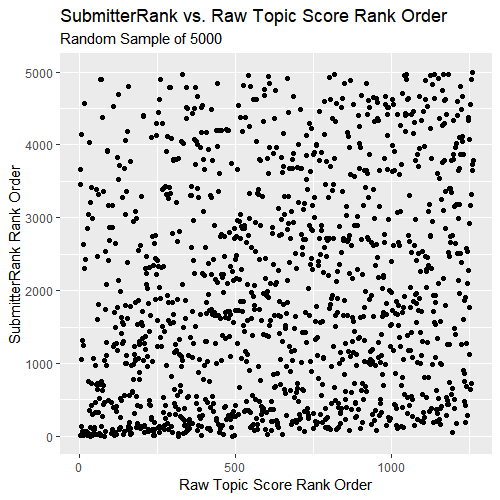
\includegraphics[width=0.45\textwidth]{rankOrder5000_orig.png} % first figure itself
        \caption{SubmitterRank vs. Raw Topic Score Rank Orders: Uniform scatter shows no relationship between the raw topic score order and the SubmitterRank order.}
	  \label{fig:5000cor_orig}
    \end{minipage}
 \end{figure}

The five submitters with the highest raw topic scores do appear to be somewhat likely to be interested in film-related opportunities, with two having submitted to film opportunities in the past, and the other three being photographers or visual artists. The five submitters with the highest SubmitterRank scores, on the other hand, are all writers with a specific interest in poetry. While this is not the desired outcome, the importance of connectivity between users in calculating their SubmitterRank scores will always tend to clump similar users, as discussed above, and so this result is not particularly surprising.

\section{Methodology Adjustments}

One possible explanation for the under-performance of the SubmitterRank seen above is that the topic scores were not weighted heavily enough. In fact, when looking at the top-ranking submitters who were not film-related, they are all very active submitters and thus would be ranked highly by a non-topic-specific SubmitterRank method. As originally designed in Section \ref{scoring}, a common submission between two users is worth one point, whether or not the opportunity has any topic-specific keywords. This means that a totally unrelated submission is worth almost as much as a submission to an opportunity with only one or two matching keywords, and users who have made a lot of submissions to opportunities will be ranked relatively highly, whether or not they are related to the topic in question.

To explore this issue further, topic scores were doubled and quadrupled for the 5000-user sample before re-running the SubmitterRank algorithm. Although the correlations between the SubmitterRank and the raw topic scores were not greatly affected (now with only about 370 of the 1000 highest-ranking users also included in the keyword-matching lists), a spot check of the five submitters with the highest SubmitterRank scores shows definite improvement in the relevance of the results. The top five submitters were the same for both the doubled and quadrupled topic scores, and now consisted of three filmmakers and two documentary-photographers. 

Another possible adjustment that would theoretically affect the influence of the topic scores on the resulting submitter ranks is changing the value of the damping factor. The way that SubmitterRank is currently designed, an increase in the damping factor would increase the influence of the opportunity topic scores, and a decrease would increase the influence of the user topic scores. \citeA{heidemann_klier_probst_2012} found that changing the damping factor only had a very slight effect on the highest ranking results, which was also found in our results. Maintaining the doubled weighting of the topic scores, the value of the SubmitterRank scores and the order of the results did change with a change in the damping factor, but overall membership in the top 1000 submitters changed very little. After increasing the damping factor ($d = 0.95$), 942 of the top 1000 submitters were still in the top 1000, and after decreasing the damping factor ($d = 0.5$), 898 of the top 1000 submitters were still in the top 1000.

\chapter{Conclusion} 

The goal of this project was to improve upon the current methods used at Submittable to identify users who may be interested in specific opportunities. It's difficult to say whether the results found above are an improvement on the current methods, but we can confidently say that the two methods provide different results, which is almost as important. If SubmitterRank resulted in a list of users that only differed very slightly from that created by straight keyword-matching, it would not be worth the additional computational and infrastructure requirements to change the current methods. Additionally, while the comparison is coarse, examining the top five submitters from the SubmitterRank and raw topic score lists suggests that the SubmitterRank algorithm may be identifying more relevant submitters. With the limitations in scope and available resources for this project, these results provide a promising starting point for further research and development of the SubmitterRank methods.

\section{Limitations}

In addressing submitter segmentation, the biggest limitation has been the vast amount of data to be processed and the time and resources necessary to do so. This was the case when exploring more traditional segmentation methods \cite{marbut_2018}, and continued to be the case with this SubmitterRank project. It may still be possible to write a script that would create the transition matrices and perform iterative multiplication on them in batches such that memory and processing power is no longer a limitation, but without major modifications to the original code, this process was estimated to take several months if performed on all 400 thousand eligible submitters. While currents methods may be sufficient for a one-off calculation, such as for research alone, this is not at all practical for the intended purposes, which would need to be completed on a 24-hour timetable at most.

Without being able to use the entire dataset of eligible submitters, we are also unable to make meaningful assertions about the efficacy of the SubmitterRank adaptation. The strength behind SubmitterRank comes largely from its ability to rank users based on their connectivity with other users in the Submittable network. However, if only a part of the network is used to build these ranks, we cannot truly know how the users would be ranked in the context of the entire network -- the presence or absence of a few highly topical users might change the entire rank order. Furthermore, we cannot measure the actual performance of a marketing campaign sent to a list created by SubmitterRank on only a sample of users for two reasons: 1. Submittable's clients expect marketing services to reach as many users as are likely to be interested (and not to be limited to a random sample); 2. The performance of this sample list would be measured in comparison to that of a keyword-matching list created from the entire bank of eligible users, and thus would not truly be comparable.

Finally, it is necessary to acknowledge that the SubmitterRank algorithm still relies on an imperfect list of topic-specific keywords. As such, the results are still susceptible to error based on the choice of these keywords. For example, the results from our 5000-user sample captured quite a few photo-journalists. This seems to indicate a failure of the algorithm, however closer inspection shows that most of these users  were matched on the word ``documentary". Since ``documentary" is on the list of film-related keywords used to create topic scores, the inclusion of these photo-journalists is due to the imprecision of the keywords and not the fault of the algorithm. In this way, an algorithm based on keywords will never be as accurate as asking users to self-identify their interests.
    
\section{Future Directions}

The first step in moving forward with this project is to find a solution for running the algorithm on the entire dataset of eligible submitters. Although we don't have a really solid way of measuring the success of our sample results, the method does seem to be performing as expected, with some indication of out-performing the current methods being used at Submittable. If nothing else, this provides enough evidence to merit further research and an attempt to include all eligible users. Currently, we are considering using a distributed computing solution, such as Hadoop or Apache Spark, to spread out the resource-heavy computational steps in the algorithm.

Once the algorithm can be run on the entire dataset, we have several options for measuring the efficacy of SubmitterRank. These methods will likely include a comparison of performance of marketing campaigns sent to lists created by the current keyword-matching methods and by SubmitterRank. Measures of performance may include e-mail open rates, click-through rates, and even actual submission rates. In addition to a straight comparison of performance, we will also likely perform logistic regression to determine whether SubmitterRank scores, raw topic scores, or straight keyword-matching are a better predictor of those same performance measures (open, click-through, and submission rates).

As mentioned above, it's also possible that Submittable will decide to ask users to self-identify their interests. In this case, we will need to explore first whether it's still necessary to use an alternative method, such as SubmitterRank, to infer user interests, or whether the self-identification makes this issue moot. If it's determined to still be helpful, the topic-scoring will need to be adjusted to either include these interests or have the interests replace the keyword-based topic scores altogether.

\bibliography{biblio}
\bibliographystyle{apacite}

%\appendix
%\addcontentsline{toc}{chapter}{Appendix}
%\section{Usecase Labels}
\chapter{Appendix A: Usecase Labels}
\label{app:usecase}
\begin{minipage}{0.5\textwidth}
\small
\centering
\begin{tabular}{rl}

  \hline
 & Usecase \\ 
  \hline
1 & Publishing \\ 
  2 & Other \\ 
  3 & Admissions \\ 
  4 & Scholarships \\ 
  5 & Job applications \\ 
  6 & Fellowship \\ 
  7 & Festival or Event \\ 
  8 & Peer Review \\ 
  9 & Artwork submissions \\ 
  10 & Audition \\ 
  11 & Grant applications \\ 
  12 & Contest or Campaign Entries \\ 
  13 & Video/Audio submissions \\ 
  14 & Award/ Nomination \\ 
  15 & Contest \\ 
  16 & Grants \\ 
  17 & Conference \\ 
  18 & Exhibition \\ 
  19 & Residency \\ 
  20 & Manuscript/Content submissions \\ 
  21 & Internal Use \\ 
  22 & Fellowship applications \\ 
  23 & Internships \\ 
  24 & Festival or Event submissions \\ 
  25 & Corporate Giving \\ 
  26 & Conference submissions \\ 
  27 & General applications \\ 
  28 & Audition submissions \\ 
   \hline
\end{tabular}
\end{minipage}

\newpage
%\section{Discover Labels}
%\label{app:discover}
\chapter{Appendix B: Discover Labels}
\begin{figure}[h]
\scriptsize
\begin{minipage}[h]{0.24\textwidth}

\begin{tabular}{rl}
  \hline
 & Discover.Label \\ 
  \hline
1 & interviews \\ 
  2 & book \\ 
  3 & review \\ 
  4 & art \\ 
  5 & fiction \\ 
  6 & prose \\ 
  7 & literary \\ 
  8 & short-story \\ 
  9 & video \\ 
  10 & submishmash \\ 
  11 & nonfiction \\ 
  12 & memoir \\ 
  13 & essay \\ 
  14 & stories \\ 
  15 & travel \\ 
  16 & visual-art \\ 
  17 & creative-writing \\ 
  18 & scripts \\ 
  19 & contest \\ 
  20 & theme \\ 
  21 & publishing \\ 
  22 & manuscript \\ 
  23 & science-fiction \\ 
  24 & drawing \\ 
  25 & painting \\ 
  26 & photography \\ 
  27 & nonprofit \\ 
  28 & chapbook \\ 
  29 & lyrics \\ 
  30 & critique \\ 
  31 & sculpture \\ 
  32 & classes \\ 
  33 & experimental \\ 
  34 & blog \\ 
  35 & for-sale \\ 
  36 & monologue \\ 
  37 & design \\ 
  38 & sports \\ 
  39 & podcast \\ 
  40 & academic \\ 
  41 & television \\ 
  42 & sound \\ 
  43 & collaborative \\ 
  44 & international \\ 
    45 & graphic-novel \\ 
  \hline
\end{tabular}
    \end{minipage}
\begin{minipage}[h]{0.24\textwidth}

\begin{tabular}{rl}
  \hline
 & Discover.Label \\ 
  \hline

  46 & article \\ 
  47 & short-play \\ 
  48 & theater \\ 
  49 & erotica \\ 
  50 & job \\ 
  51 & science \\ 
  52 & criticism \\ 
  53 & hybrid \\ 
  54 & dance \\ 
  55 & student \\ 
  56 & exhibition \\ 
  57 & philosophy \\ 
  58 & military \\ 
  59 & grant \\ 
  60 & native-american \\ 
  61 & children \\ 
  62 & column \\ 
  63 & health \\ 
  64 & politics \\ 
  65 & culture \\ 
  66 & social-justice \\ 
  67 & volunteer \\ 
  68 & animation \\ 
  69 & speculative \\ 
  70 & subscribe \\ 
  71 & print \\ 
  72 & festival \\ 
  73 & multilingual \\ 
  74 & comedy \\ 
  75 & humor \\ 
  76 & conference \\ 
  77 & retreat \\ 
  78 & environmental \\ 
  79 & scholarships \\ 
  80 & public-art \\ 
  81 & cover-art \\ 
  82 & independent \\ 
  83 & workspace \\ 
  84 & art-fair \\ 
  85 & african-american \\ 
  86 & paranormal \\ 
  87 & juried \\ 
  88 & season \\ 
  89 & asian-american \\ 
  90 & alcohol \\ 
  
  \hline
\end{tabular}
    \end{minipage}
\begin{minipage}[h]{0.24\textwidth}

\begin{tabular}{rl}
  \hline
 & Discover.Label \\ 
  \hline
  91 & fashion \\ 
  92 & midwest \\ 
  93 & VR/360 \\ 
  94 & female \\ 
  95 & VR \\ 
  96 & public-media \\ 
  97 & civil-rights \\ 
  98 & mental-health \\ 
  99 & journal \\ 
  100 & poetry \\ 
  101 & magazine \\ 
  102 & anthology \\ 
  103 & writing \\ 
  104 & flash \\ 
  105 & feedback \\ 
  106 & short-film \\ 
  107 & screenwriting \\ 
  108 & feminist \\ 
  109 & young-adult \\ 
  110 & novel \\ 
  111 & agent \\ 
  112 & online \\ 
  113 & magical-realism \\ 
  114 & translation \\ 
  115 & adventure \\ 
  116 & award \\ 
  117 & residency \\ 
  118 & plays \\ 
  119 & haiku \\ 
  120 & community \\ 
  121 & business \\ 
  122 & funding \\ 
  123 & editor \\ 
  124 & digital \\ 
  125 & book-arts \\ 
  126 & journalism \\ 
  127 & audio \\ 
  128 & surrealist \\ 
  129 & documentary \\ 
  130 & film \\ 
  131 & mystery \\ 
  132 & technology \\ 
  133 & comics \\ 
  134 & pitch \\ 
  135 & illustration \\ 
 \hline
\end{tabular}
    \end{minipage}
\begin{minipage}{0.24\textwidth}

\begin{tabular}[h]{rl}
  \hline
 & Discover.Label \\ 
  \hline

  136 & religion \\ 
  137 & fellowship \\ 
  138 & performance \\ 
  139 & prize \\ 
  140 & romance \\ 
  141 & horror \\ 
  142 & education \\ 
  143 & lgbtqia \\ 
  144 & fantasy \\ 
  145 & food \\ 
  146 & architecture \\ 
  147 & spoken-word \\ 
  148 & indigenous \\ 
  149 & readings \\ 
  150 & media \\ 
  151 & music \\ 
  152 & canada \\ 
  153 & gallery \\ 
  154 & mythology \\ 
  155 & emerging \\ 
  156 & event \\ 
  157 & music-composition \\ 
  158 & parenting \\ 
  159 & minorities \\ 
  160 & crafts \\ 
  161 & printmaking \\ 
  162 & workshop \\ 
  163 & internship \\ 
  164 & novella \\ 
  165 & mentorship \\ 
  166 & history \\ 
  167 & ceramics \\ 
  168 & museum \\ 
  169 & orchestra \\ 
  170 & new-york \\ 
  171 & fiber-arts \\ 
  172 & paper \\ 
  173 & poster \\ 
  174 & thriller \\ 
  175 & 360-Video \\ 
  176 & tequila \\ 
  177 & service-learning \\ 
   \hline
\vspace{.82cm}
\end{tabular}

    \end{minipage}
\end{figure}


\end{document}